\documentclass[11pt, letterpaper]{report}

\usepackage{color, soul}
\usepackage[dvipsnames]{xcolor}
\usepackage{amsmath}
\usepackage{kpfonts}
\usepackage{inconsolata}
\usepackage[T1]{fontenc}
\usepackage{listings}
\usepackage{titlesec}
\usepackage{graphicx}
\usepackage{changepage}
\usepackage{minted}

\lstset{basicstyle=\ttfamily\footnotesize}

\DeclareGraphicsExtensions{.jpg, .png}

\begin{document}

\title{Data Mining Assignment 3}
\author{Ryan Case}
\date{\today}
\maketitle{}

\section{ID3 and Weather Data}

\subsection{Methodology}

The weather data set is a set of 14 instances with attributes corresponding to weather conditions. The dependent variable is \texttt{play}, whose value denotes whether or not a sporting event should take place given the weather conditions.

Given the small number of observations there is a high likelihood that inaccuracies will be introduced by splitting the data into training and testing. Instead I used K-Fold cross validation to maximize the number of instances used for training, while still getting a good idea of how the classifier would generalize to more data. The classifier is an ID3 decision tree.

\subsection{Results}

\begin{tabular}{ |l l l| }
    \hline
    \textbf{K} & \textbf{Accuracy} & \textbf{Kappa} \\ \hline
    5 & 71.43\% & 0.4286 \\
    10 & 85.71\% & 0.6889 \\
    14 & 78.57\% & 0.5116 \\
    \hline
\end{tabular}

\bigskip
\subsection{Conclusions}

One problem with assessing the data for this is once again the size of the data set. 10-fold and 14-fold only differ by a single misclassification but it is enough to change the accuracy rating by over 7\%.

It's hard to predict how these results would generalize to a larger data set, or how the accuracy number would compare to a classifier trained on more data. It's likely that more observations would reinforce patterns that and improve accuracy. On the other hand there are only 36 possible combinations of the independent variables, so more observations could offer only marginal improvements if the data is noisy. Similarly our tree may have captured the fundamental patterns in our data, or it may have overfit to noise.

Overall though, ID3 and cross validation seems to be a good approach to this problem. 85.71\% accuracy is an impressive number given such a small number of examples and suggests that the underlying pattern has been captured here.

\section{Breast Cancer Data Imputation}

\subsection{Methodology}

To impute missing values I chose a KNN instance-based imputation method. Compared to other common missing value strategies like dropping instances with null values or filling them with a class value like the mean or median, instance-based imputation should offer greater granularity and won't reduce the size of the dataset or change its distribution.

I felt KNN was ideal for several reasons. First, it requires virtually no training time and only needs to classify $n$ missing values, where $n$ is the total number of missing values. Second, it is robust and adaptable to the needs of the problem. The distance function can be made to handle missing values, categorical or numeric values, it can normalize on the fly, it can weigh different attributes differently, etc. Essentially the distance function can be easily tweaked to suit any dataset.

A weakness of KNN for imputation would arise if the attribute being imputed were extremely noisy and without a clear decision boundary, or with a very complicated decision boundary. KNN is poorly suited to such situations.

For this particular dataset every variable is treated as categorical and very few values are missing overall. For the distance function I treated all disagreements between two instances as equivalent to a distance of 1, agreement equivalent to a distance of 0, and instances with any missing values were simply ignored. The code for the implementation follows:

\begin{minted}[fontsize=\footnotesize]{py}
import numpy as np
import pandas as pd
from math import isnan

def impute_neighbors(row, n_neighbors=3):
    """
    Uses KNN for data imputation. Accepts only categorical values and ignores
    rows with any null values. Returns the k-nearest instances as a dataframe
    """
    neighbors = []
    for i, instance in data.iterrows():
        # Iterate over all the rows in the dataframe
        if row.name == i or instance.isnull().any():
            # If we're looking at the same row we passed or a row
            # with null values we pass over this instance
            continue
        else:
            # Otherwise measure the distance
            dist = 0
            for attr, _ in row.iteritems():
                # Distance is 1 if the two items are not equal, 0 otherwise
                if row[attr] != instance[attr]:
                    dist += 1
            # Append the distance and instance to our list
            neighbors.append((dist, instance))
    # Sort the list by distances and store only the instances
    knn = [tup[1] for tup in sorted(neighbors, key=lambda t: t[0])]
    # Return the KNN as a dataframe
    return pd.DataFrame(knn[:n_neighbors], columns=row.index)


def knn_impute(data, k_neighbors=3):
    """
    Imputes missing data using the nearest non-null neighbors
    """
    # Iterate over rows
    for i, row in data.iterrows():
        # Find rows that contain nulls
        if row.isnull().any():
            # Find K nearest neighbors
            knn = impute_neighbors(row)
            # Find the cell with the null value and fill it
            for i, v in row.iteritems():
                if isinstance(v, float) and isnan(v):
                    # Fill that with the voted upon value
                    val = knn[i].mode().values[0]
                    data.set_value(row.name, i, val)
\end{minted}

I will be comparing this implementation to two other approaches: Deleting all instances with missing values and filling the missing values with a class value such as the median or mode. The first is accomplished by copying and deleting rows with missing values from the arff file. The second can be accomplished through the Weka filter \texttt{ReplaceMissingValues}. All of them will use an ID3 decision tree with 10-fold cross validation, and to check for overfitting the training score will be calculated by running training and testing both on the entire data set.

\subsection{Results}

\begin{tabular}{ |l l l l| }
    \hline
    \textbf{Dataset} & \textbf{Training Accuracy} & \textbf{CV Accuracy} & \textbf{CV Kappa} \\ \hline
    No Imputation & 97.83\% & 58.84\% & 0.1349 \\
    Class-Based Imputation & 97.90\% & 56.99\% & 0.0906 \\
    Instance-Based Imputation & 97.90\% & 55.94\% & 0.0697 \\
    \hline
\end{tabular}

\subsection{Conclusions}

All three approaches turned in a fairly mediocre classification performance of under 60\%. The dataset in which instances with missing values were removed performed better than the two in which values were imputed and of the two imputed datasets the class-based approach performed better than the instance-based approach. Finally, all three datasets have relatively abysmal Kappa scores.

So what happened and why did the instance-based approach unexpectedly perform the worst? The answer is suggested by the training score. Our KNN imputation approach performs over 40\% better on training data than it does on testing data, a massive gulf. Such a difference is the hallmark of a model that is overfitting. Sure enough, a look at the generated tree reveals a deep tree with very complex rules, another symptom of this.

This issue turns out to be the Achilles Heel for our approach because an overfitting model gains too much information from the noise, while data imputation invariably adds noise to the data because it cannot perfectly predict all imputed values. So a tree that overfits to our imputed data stands a good chance of not generalizing well, on top of the normal problems that come from overfitting.

When we change the predictor to a C4.5 tree the overfitting disappears and all three datasets perform equivalently with the imputed sets performing the best, and KNN imputation getting a slight edge over the class-based approach. The issue then seems to lie with the model more than the imputation method.

\section{ID3 Generalization}

\subsection{Methodology}

To look at ID3's ability to generalize I will be running 9 different splits between the training and testing data. Starting at 10\% train and 90\% test the ratios will change by +10\%/-10\% every iteration. Finally, for comparison I will also be running 10-fold CV and using 100\% of the set for both training and testing.

Every split will be tested on 5 randomizations of the data set, labeled $R_{1}$ through $R_{5}$, with the mean of those is represented by $R_{M}$. The soybean dataset is missing values and those will be filled using Weka's built in replacement heuristic which uses class values for imputation. The standard deviation of each set is also included. The means of each split are graphed to give a better visual representation to array of numbers generated by this testing method.

\subsection{Results}

\begin{tabular}{ |l|l|l|l|l|l|l||l|l| }
    \hline
    \% Train & \% Test & $R_{1}$ & $R_{2}$ & $R_{3}$ & $R_{4}$ & $R_{5}$ & $R_{M}$ & $\sigma$ \\ \hline \hline
    10\% & 90\% & 50.24\% & 53.50\% & 42.76\% & 45.04\% & 39.18\% & 46.14\% & 5.75 \\ \hline
    20\% & 80\% & 68.68\% & 65.02\% & 73.63\% & 64.29\% & 70.15\% & 68.35\% & 3.83 \\ \hline
    30\% & 70\% & 73.85\% & 76.57\% & 62.34\% & 73.22\% & 76.78\% & 72.55\% & 5.92 \\ \hline
    40\% & 60\% & 74.15\% & 80.73\% & 80.98\% & 80.24\% & 76.10\% & 78.44\% & 3.12 \\ \hline
    50\% & 50\% & 82.40\% & 79.47\% & 77.71\% & 83.87\% & 83.58\% & 81.41\% & 2.70 \\ \hline
    60\% & 40\% & 84.24\% & 86.08\% & 87.91\% & 86.81\% & 85.25\% & 86.10\% & 1.41 \\ \hline
    70\% & 30\% & 81.46\% & 87.80\% & 88.78\% & 85.85\% & 87.32\% & 86.24\% & 2.87 \\ \hline
    80\% & 20\% & 92.70\% & 86.13\% & 87.59\% & 87.59\% & 84.67\% & 87.74\% & 3.03 \\ \hline
    90\% & 10\% & 83.82\% & 91.18\% & 94.12\% & 94.12\% & 88.24\% & 90.23\% & 4.36 \\ \hline
\end{tabular}

\bigskip
\begin{tabular}{ |l|l| }
    \hline
    \textbf{Alternate Validation} & \textbf{Accuracy} \\ \hline
    10-Fold CV & 89.17\% \\ \hline
    No Split & 99.85\% \\ \hline
\end{tabular}

\bigskip
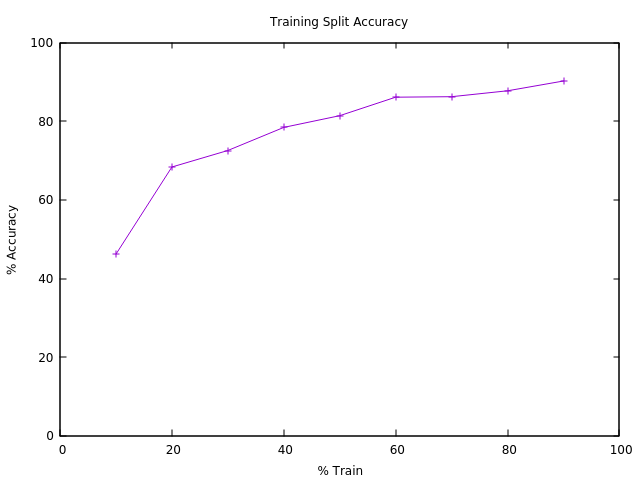
\includegraphics[scale=0.75]{train_split_graph}

\subsection{Conclusions}

Plenty of numbers in the results here but the general trend is best represented by the graph. The larger the training set the more accurately our tree was able to generalize to unseen data. The steepest gains occurred between 10\% and 20\% of the data being used for training, but gains were seen all the way up to 90\%. Looking at our other validation methods we see approximately 90\% accuracy for cross validation so it suggests that our final results are accurate. Once again when we use 100\% of the data for training and testing we get an extremely high accuracy of over 99\%, which is a sign that the model overfits, but accuracy of 90\% on unseen data is still a good result.

Somewhat surprisingly the standard deviation for the sets did not decrease as markedly as I expected. Even when using a large training set the effect of the random split was enough to change the accuracy of the results by as much as 10\%. The tendency of ID3 to overfit is doubtless responsible for some of this, but regardless it reinforces the importance of comprehensive evaluation of a model and not just blindly accepting the highest accuracy number you generate.

\section{Iterative ID3 Training}

\subsection{Methodology}

To test the approach of training an ID3 tree by specifically training on failed instances rather than simply a random subset of instances I will be using the soybean data set. First the missing values are imputed using the Weka class-value approach. Next the dataset is randomized and split into 20\% train / 80\% test. At each iteration I will record the accuracy and move 10 failed instances from the training set to the testing set. I am using two metrics for when to stop the iterations:

\begin{enumerate}
    \item{If the accuracy of the training set moves to within $\frac{+}{-}5\%$ of the 10-fold cross validation score of 87.55\%}
    \item{After 70 observations have been added to the dataset, which corresponds approximately to a 30\% train / 70\% test split.}
\end{enumerate}

Whichever comes first. Either condition should be enough to show whether a small, selective data set can offer equivalent performance to a much larger, non-selective set. Finally, for comparison I will graph the performance of this approach versus adding approximately the same number of instances to the training set using splits of randomized data.

\subsection{Results}

\begin{tabular}{ |l|l|l|l| }
    \hline
    \textbf{Train Size} & \textbf{Accuracy} & \textbf{$\Delta$ Prev.} & \textbf{$\Delta$ CV} \\ \hline
    137 & 65.39\% & N/A & -22.16\% \\
    147 & 71.46\% & +6.07\% & -16.09\% \\
    157 & 74.71\% & +3.25\% & -12.84\% \\
    167 & 79.65\% & +4.95\% & -7.89\% \\
    177 & 77.67\% & -1.98\% & -9.88\% \\
    187 & 78.63\% & +0.96\% & -8.92\% \\
    197 & 80.04\% & +1.41\% & -7.51\% \\
    207 & 80.88\% & +0.84\% & -6.67\% \\
    \hline
\end{tabular}

\bigskip
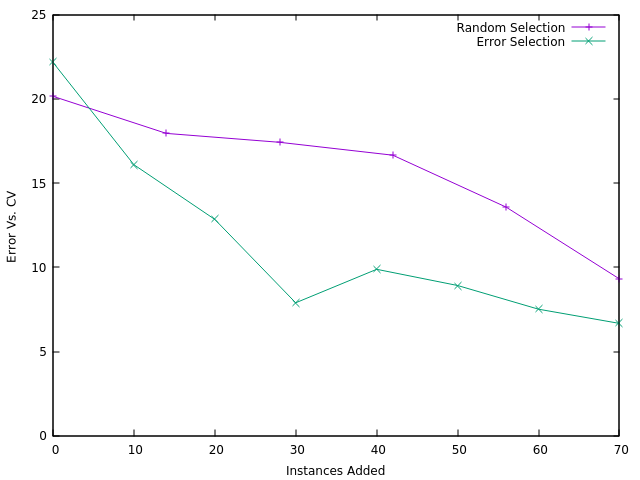
\includegraphics[scale=0.75]{random_vs_error_selection}

\pagebreak
\subsection{Conclusions}

The accuracy gain from the first few iterations of this approach are truly impressive.With only 30 instances added the accuracy jumps from 65\% to 79\% and the error versus using the whole data set in cross-validation goes down to less than 10\%. Graphing this against adding similar numbers of elements randomly shows that intentionally selecting errors reduces the error rate faster than random selection. Overall the approach lives up to its claims of training the tree more efficiently compared to random splits.

Having said that, while the gains are notable they aren't decisive. Both approaches have aberrant situations where their accuracy actually goes down with more instances, and ultimately the error from random selection is not significantly worse than choosing them intentionally. If the goal is to get by with a much smaller dataset than random selection allows, it's not clear that this method can really achieve that consistently. To make matters worse you can only choose failed observations once you know they have failed so this approach requires iterative training rather than training potentially just once, making it less time efficient.

Still, it seems to be a useful tool for extremely large datasets if you can automate the approach. Being able to start with 10-20\% of the data and intelligently build the training set from the failed examples could save time, space and energy. Given that datasets are not typically getting any smaller that's a good tool to have.

\end{document}
